\section*{How to reach the lecture rooms}
\addcontentsline{toc}{section}{How to reach the lecture rooms}
The Conference has several locations: it will open in Aula magna Santa Lucia (via Castiglione 36).
Then on Tuesday 5 June afternoon and in the other days it will take place in:

\bigskip

\begin{itemize}
\item Building A and Building B - Room A, B, C, D, E, F, G, H, I, L, M, N, O, P, Q (via Belmeloro 14)
\item SP.I.S.A - Aula magna (via Belmeloro 12)
\item Redenti - Room 1 and Room 2 (via Belmeloro 10)
\item Matemates
\end{itemize}

\bigskip

\noindent The following map shows the location of these buildings:

\bigskip

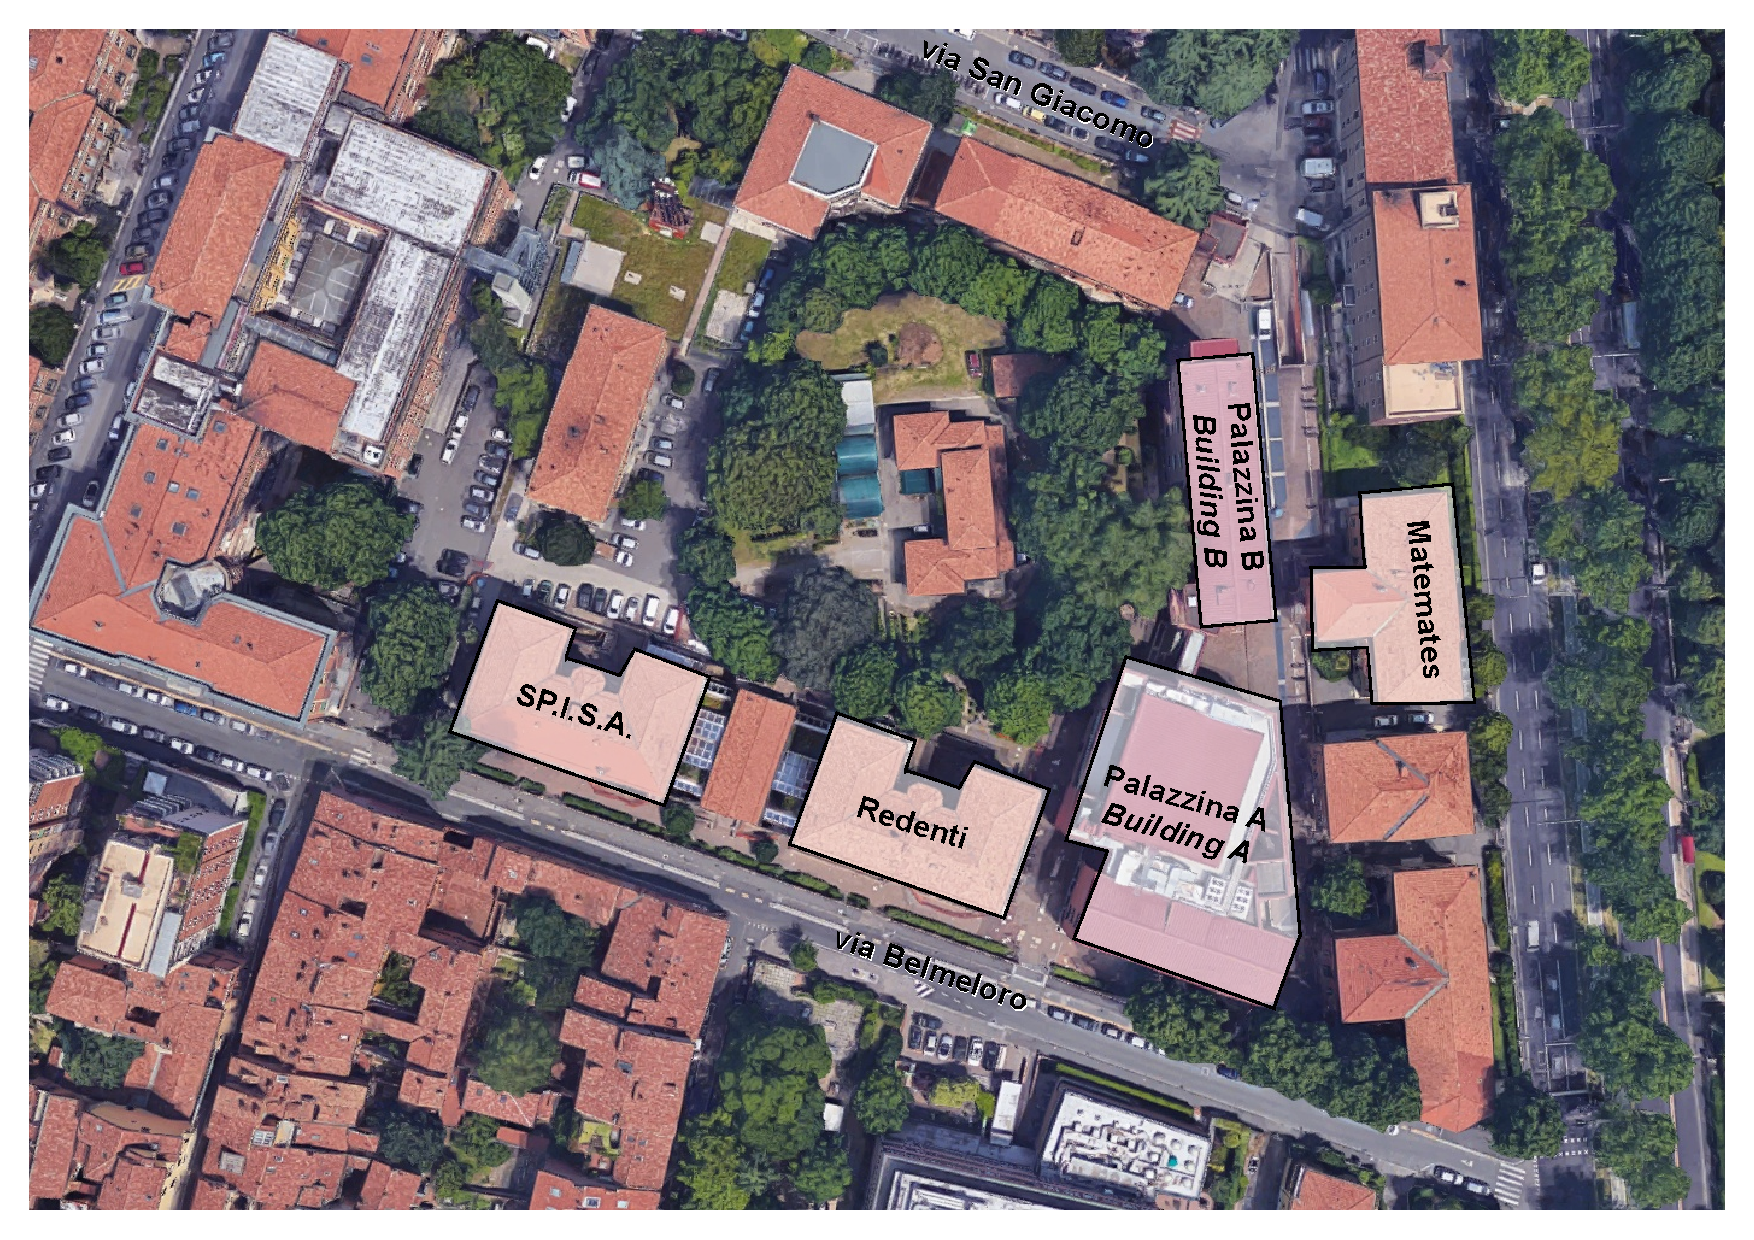
\includegraphics{satellite.jpg}

\newpage

\includegraphics[width=16cm]{images/maps/f01-Belmeloro14_p0.png}

\vspace{2cm}

\includegraphics[width=16cm]{images/maps/f02-Belmeloro14_p1.png}

\newpage

\includegraphics[width=16cm]{images/maps/f03-Belmeloro14_p2.png}

\vspace{2cm}

\includegraphics[width=16cm]{images/maps/f04-Belmeloro14_p3.png}

\newpage

\includegraphics[width=16cm]{images/maps/f05-Belmeloro10-12_p0.png}

\vspace{2cm}

\includegraphics[width=16cm]{images/maps/f06-Belmeloro10-12_p1.png}

\newpage

\begin{multicols}{2}
%-----Registration Desk
\section*{Registration Desk}
\addcontentsline{toc}{section}{Registration Desk}
The registration desk is located in the hall of Building A, via Belmeloro 14 and is open during the following hours:
\begin{itemize}
\item Monday, June 4: 3:00 PM - 6:30 PM
\item Tuesday, June 5: 11:30 AM - 6:30 PM
\item Wednesday, June 6: 8:00 AM - 6:30 PM
\item Thursday, June 7: 8:00 AM - 6:30 PM
\item Friday, June 8: 8:00 AM - 6:30 PM
\end{itemize}
%-----Badges
\subsection*{Badges} Carry your badge during the conference so that you can be admitted to all technical sessions, coffee breaks, lunches, reception and banquet.\\
Emergency numbers are provided on the back of your name badge! 
%-----Registration Fee Includes
\subsection*{Registration Fee Includes}
\begin{itemize}
\item Admission to all technical sessions
\item Business Meeting (open to SIAG/IS members)
\item Social Dinner
\item Coffee breaks 
\item Welcome Lunch 
\item Welcome cocktail during the evening Poster Session
\item Room set-ups and audio/visual equipment
\item Wi-Fi access at the conference
\end{itemize}%-----Conference Talk Arrangements
%-----Conference Talk Arrangements
\subsection*{Conference Talk Arrangements}
All plenary talks will have a slot of 45 minutes
(5 minutes reserved for questions and discussion included).\\\\
The minitutorials will last 2 hours.\\\\
All minisymposia talks will have a slot of 30 minutes (5 minutes reserved for questions and discussion included).
All contributed talks will last 20 minutes (5 minutes reserved for questions and discussion included).\\\\
If you need to copy your presentation slides from your USB to a
computer in lecture hall or meeting room, please do it in advance before
the session starts.
%-----Important Notice to Poster Presenters
\subsection*{Important Notice to Poster Presenters}
The poster sessions are scheduled:
\begin{itemize}
\item Tuesday, June 5 from 6:30 PM onwards in Building A, with Welcome cocktail;
\item Wednesday, June 6 from 11:30 AM - 1:00 PM in Building A.
\end{itemize} 
The Best Poster Award will be assigned on Friday, June 8 at 1:00 PM in Building A, Room A.\\
All posters participating to the Best Poster Award are available on the Conference website from June 1.\\
Poster presenters are requested to set up
their material on the provided poster boards (70 cm x 100 cm), following the indication in the participant folder and be present during both sessions.  
All materials must
be posted by Tuesday, June 5 at
6:00 PM.
The conference is not responsible for
discarded posters.
%------------Wi-Fi Access
\section*{Wi-Fi Access}
The username and password of your account during the conference period (5-8 June) can be found in your folder.
%-------------------Standard Audio/VIsual Set-Up in Meeting Rooms
\subsection*{Standard Audio/Visual Set-Up in Meeting Rooms}
The plenary session room has a PC, two screens and two data projectors.\\ 
All other concurrent/breakout rooms have a PC, a screen, a data projector and a whiteboard (overhead projectors are also available).\\
The data projectors support VGA connection only. Presenters requiring an HDMI or alternate connection must provide their own adaptor.\\
Cables or adaptors for Apple computers are not supplied, as they vary for each model: please bring your own cable/adaptor if using a Mac computer. 
The conference is not responsible for the safety and security of speakers' computers.\\
%-------------Recording of presentations
\subsection*{Presentations Recording}
During the conference audio and video recording is prohibited without the written permission of the speaker and the conference.
%-------------SIAM Books and Journal
\subsection*{SIAM Books and Journals}CHIEDERE
Display copies of books and complimentary copies of journals are available on site. SIAM books are available at a discounted price during the conference. The book booth will be staffed from 9:00 AM through 6:00 PM. \\If a SIAM books representative is temporarily away from the booth, completed order forms and payment (credit cards are preferred) may be taken to the registration desk. The books table will close at 4:00 PM on Friday??? (2016)\\
Completed order forms should be emailed or faxed to the SIAM office directly. It is not allowed to carry out on site transaction during the conference period??? (2014)
%------------------ GET TOGETHERS
\addcontentsline{toc}{section}{Get-togethers}
\subsection*{Get-togethers}
\begin{itemize}
\item Tuesday, June 5, 11:45 AM - 1:30 PM, Welcome Lunch
\item Tuesday, June 5, 6:30 PM - 8:30 PM, Poster Session I and Welcome cocktail
\item Wednesday, June 6, 11:30 AM - 1:00 PM, Poster Session II
\item Wednesday, June 6, 5:45 PM - 6:30 PM Business meeting
\item Wednesday, June 6, 8:00 PM Social dinner
\end{itemize}
%---------------Lunches
\subsection*{Lunches}
There are different solutions for your lunches on Wednesday, Thursday and Friday. 
\begin{itemize}
\item Two different lunch baskets prepared by the catering in the conference location: it can be ordered at the coffee desk the day before.
\item The John Hopkins University canteen in front of the conference location: please show your conference badge.
\item Elior canteen, Piazza Vittorio Puntoni 1: special rates for the conference participants.
\end{itemize}
Several bars and restaurants are available for lunch in the area surrounding via Belmeloro: the complete list is in your folder.

%---------------Conference Banquet
\subsection*{Conference Banquet}
The Conference banquet will be served in Palazzo Re Enzo, in Piazza del Nettuno 1C: please carry your badge with you\\ Additional conference banquet tickets are available at the price of 65 euros. Please buy it at the registration desk before Tuesday, June 5 afternoon.\\ For PhD students a special dinner is organized in the same evening at................
%---------------Child Care
\subsection*{Child Care}
\begin{itemize}
\item \emph{Le cicogne} (http://www.lecicogne.net/)\\
Indicative rates: if reserved a few days in advance: \euro 16 / each hour (for a maximum of 2-3-4 hours) for a basic Baby Sitting and \euro 20/each hour for a Baby Sitter speaking foreign languages.
If requested one day before: \euro 18 + hourly rate.
If requested the same day: \euro 28 + hourly rate.
\item \emph{Born to life} (http://www.bolognababysitter.it/)\\
Indicative rates: \euro 25 agency fee + hourly rate \euro 13 . After 10 PM: \euro 15 Foreign languages available. Reservations: 2 weeks in advance.
\end{itemize}
%---------------Please Note
\subsection*{Please note}
The conference is not responsible for the safety and security of participants' computers. Do not leave your laptop computers and personal belongings unattended. Please remember to turn off your mobile during all the sessions.\\\\ The conference cannot provide photocopying and dollar exchange service. A bank can be found in piazza Aldrovandi 12/A (opening hours: 8:20 AM-1:20 PM and 2:30 PM-4:00 PM).
%---------------Comments
\subsection*{Comments?}
Comments about SIAM IS18 are encouraged! Please send it to Cynthia Phillips, SIAM Vice President for Programs (vpp@siam.org)
\end{multicols}
